\documentclass[12pt]{article}
\usepackage[utf8]{inputenc}
\usepackage{amssymb}
\usepackage{wasysym}
\usepackage[a4paper, margin=2cm]{geometry}
\usepackage[dvipsnames]{xcolor}
\usepackage{graphicx}
\graphicspath{ {./PoC Scoping Exercise/} }
\usepackage{scrextend}

\title{\textbf{Learning Journal}}
\date{\today}
\author{William Black 42920477}
\setlength{\parindent}{0pt}
\setlength{\parskip}{0.5em}

\usepackage{hyperref}
\hypersetup{
    colorlinks=true,
    linkcolor=blue,
    filecolor=magenta,      
    urlcolor=cyan,
}
 
\urlstyle{same}
 
\begin{document}
    \maketitle\textbf{\large{11.08.19 – Scoping Exercise}}\par

Doing the Scoping Exercise first because the other task is recommended to be tackled in groups

Time to find out how to use LaTeX

First learning journal will be in Word since I don’t know how to use LaTeX yet

Brian said to work in Rich Text and watch it come out perfectly on the right

\begin{itemize}
\renewcommand{\labelitemi}{$\nobullet$}
\item \underline{Problems:}
\renewcommand{\labelitemi}{$\bullet$}
    \item It does not come out perfectly on the right at all
    \item Sometimes code appears on the Rich Text version of the left
    \item The rich text options are extremely limited, it seems to just be bold, underline, bullet lists, and nothing else
\end{itemize}

\begin{itemize}
\renewcommand{\labelitemi}{$\nobullet$}
\item \underline{Solution:}
\renewcommand{\labelitemi}{$\bullet$}
    \item Don’t use Rich Text mode
\end{itemize}

Brian linked a \href{https://www.overleaf.com/learn/latex/Creating_a_document_in_LaTeX}{tutorial} for using Source mode

Tutorial going smoothly

Replacing parts of the tutorial result to reflect my Scoping Exercise

Worked out using $\backslash$date\{$\backslash$today\} instead of typing out the date, magic!

\begin{itemize}
\renewcommand{\labelitemi}{$\nobullet$}
\item \underline{Problem:}
\renewcommand{\labelitemi}{$\bullet$}
    \item Can’t work out how to make nested bullets.
\end{itemize}
\begin{itemize}
\renewcommand{\labelitemi}{$\nobullet$}
\item \underline{Solution:}
\renewcommand{\labelitemi}{$\bullet$}
    \item \href{https://www.overleaf.com/learn/latex/Lists}{This tutorial} shows how to make nested bullets. Since I can, as a learning exercise, I want to combine bullets, bullets, and numbered lists.
\end{itemize}

I’m numbering the parts of my methodology, including the writing process and the bibliography creation. The pains and pain relievers can be bullets.

\href{https://www.overleaf.com/learn/latex/Lists}{The same tutorial} even shows how to change bullet list styles

\href{http://www.rpi.edu/dept/arc/training/latex/LaTeX_symbols.pdf}{This .pdf} is a list of different symbols I can use. 

\begin{itemize}
\renewcommand{\labelitemi}{$\nobullet$}
\item \underline{Problem:}
\renewcommand{\labelitemi}{$\bullet$}
    \item Not working. Some of them work but most of them don’t.
\end{itemize}
\begin{itemize}
\renewcommand{\labelitemi}{$\nobullet$}
\item \underline{Solution:}
\renewcommand{\labelitemi}{$\bullet$}
    \item \usepackage{} with the package the symbol is from was surprisingly easy. I assumed I had to install something but just naming the package seems to work. 
    \item I wonder why they don’t just put something like “$\backslash$usepackage\{allpackages\}” at the beginning, and why not make that automatic?
\end{itemize}
    
Just realised I have to write gains and gain creators too, and I have the perfect bullet symbols for them. 

I kind of feel like some sort of genius hacker using LaTeX but my brain is starting to hurt, I’ve been fiddling around with the source editor for a few hours now.
There’s an option to collapse lists at the line numbers when you’re done writing them. It’s much easier to read. I’ve also realised I can separate the lines with single line breaks and nothing changes in the result, which also makes the code much more readable.

\begin{itemize}
\renewcommand{\labelitemi}{$\nobullet$}
\item \underline{Problem:}
\renewcommand{\labelitemi}{$\bullet$}
    \item Even with \href{https://www.overleaf.com/learn/latex/Text_alignment#Right-justified_text}{a tutorial} I can’t make a package work to allow me to make the date right-aligned and smaller.
\end{itemize}
\begin{itemize}
\renewcommand{\labelitemi}{$\nobullet$}
\item \underline{Solution:}
\renewcommand{\labelitemi}{$\bullet$}
    \item
\end{itemize}
    
Can’t figure out any solution to that problem so I’ll just leave it as is. I wanted to make the date a little less front-and-centre, but maybe the package isn’t working because it’s in the preamble.

But now it looks like I can change the format of the title, so that’s not the rule. \href{https://www.overleaf.com/learn/latex/Font_sizes,_families,_and_styles}{This tutorial} explains how to change font sizes, but rather than “12pt” etc it’s just larger or smaller than the size set at the beginning of the document.

Came across \href{https://www.overleaf.com/learn/latex/Paragraph_formatting#Reference_guide}{this tutorial} that tells me how to fix the automatic indenting. Looks nicer without it.

\begin{itemize}
\renewcommand{\labelitemi}{$\nobullet$}
\item \underline{Problem:}
\renewcommand{\labelitemi}{$\bullet$}
    \item The margins look kind of insane, they’re like two inches wide, and for some reason they’re even wider on only the second page. The first and third page look normal though.
\end{itemize}
\begin{itemize}
\renewcommand{\labelitemi}{$\nobullet$}
\item \underline{Solution:}
\renewcommand{\labelitemi}{$\bullet$}
    \item After a lot of messing around with this tutorial to use the geometry package to make the margins more normal, I realised two-sided letter paper was still the document style set from when I was going through the set-up tutorial. I’ve made the paper A4 and one-sided.
\end{itemize}

While I don’t think these specific skills are necessarily going to be so handy in creating the ultimate Proof of Concept submission, learning how to search for things I don’t know how to do and familiarising myself with the logic of the program has been a difficult learning curve that I’m enjoying being on top of.

I’m finding it extremely confusing, how to submit the document. Someone else in class has submitted a .tex file, and now I reread the instructions, it does say specifically to upload either a .tex file or a word file on to cloudstor, not a .pdf. But there’s no button to download a .tex file, just a .pdf.

Okay an hour later I figure out you have to exit the program, and download a .zip of the file that contains the .tex file. 

Submitted the .tex file to Cloudstor, the .pdf to Turnitin.

Fingers crossed that next week’s task will take less than 6 hours now I’m more familiar with the program

\newpage
    \maketitle\textbf{\large{12.08.19 – Data Carpentry}}\par
Since yesterday’s task was so surprisingly complicated, I might see how I do with Data Carpentry solo and keep the tricky parts to ask my friends tomorrow.

\setlength{\parskip}{1cm}

{\textbf{\href{https://datacarpentry.org/spreadsheets-socialsci/00-intro/index.html}{Introduction}}}
\setlength{\parskip}{0.5em}


\color{Gray}\textbf{{Questions}}
\newline What are basic principles for using spreadsheets for good data organization?

\textbf{{Objectives}}
\newline Understand how to organize data so computers can make the best use of the data

\begin{itemize}
\renewcommand{\labelitemi}{$\nobullet$}
\item \textbf{\underline{Exercise}}
\renewcommand{\labelitemi}{$\bullet$}
    \item How many people have used spreadsheets in their research?
    \item How many people have accidentally done something that made them frustrated or sad?
\end{itemize}\color{black}

I’ve used spreadsheets in research quite simply, just to find average values, or added values. A couple of times I tried to test for a null hypothesis, because I had just done Statistics 102 and I could still remember how to do it, but that was very complicated and I’m not 100\% confident doing it again now.

I don’t know if I’ve had that situation in the context of research… a few times a Windows update has interrupted me during an exam, which is scary, but I’ve just taken photos to prove I had a technical error. Definitely the worst one is when a Windows update restarts my computer and I’ve forgotten to save my Word file. It’s fine if you’ve saved it once, because AutoSave saves it for you, but if you haven’t saved and named it yet AutoSave doesn’t run.

\vspace{1em}
\textbf{\href{https://datacarpentry.org/spreadsheets-socialsci/01-format-data/index.html}{Formatting Data in Spreadsheets}}

\\\color{Gray}\textbf{{Questions}}
\\ What are some common challenges with formatting data in spreadsheets and how can we avoid them?

\textbf{{Objectives}}
\\Recognise and resolve common spreadsheet formatting problems.
\\Describe the importance of metadata.
\\Identify metadata that should be included with a dataset.
\color{black}

\vspace{1em}
\textbf{Data formatting} – always prioritise the computer understanding the data over you understanding it. You may need to format differently for different objectives.

\textbf{Keep track of analyses} – never clean/analyse/mess around with your original data, make a copy in a new tab/file and mess with that. Open the next tab to keep notes on what you did to end up with the new version, because you won’t remember in six months.

\textbf{Structuring data} – variables in columns, observations in rows, split all combined observations to simplest possible. When exporting cleaned data, use text-based format like comma-separated values (CSV)

\newpage
\color{gray}
\begin{itemize}
\renewcommand{\labelitemi}{$\nobullet$}
\item \textbf{\underline{Exercise}}
\item We’re going to take a messy version of the SAFI data and describe how we would clean it up.
\end{itemize}
\begin{enumerate}
    \item Download the messy data.
    \item Open up the data in a spreadsheet program.
    \item Notice that there are two tabs. Two researchers conducted the interviews, one in Mozambique and the other in Tanzania. They both structured their data tables in a different way. Now, you’re the person in charge of this project and you want to be able to start analyzing the data.
    \item With the person next to you, identify what is wrong with this spreadsheet. Discuss the steps you would need to take to clean up the two tabs, and to put them all together in one spreadsheet.
\end{enumerate}
\color{black}

\begin{enumerate}
    \item Downloaded.
    \item Opened.
    \item Noticed tabs.
    \item There are too many things wrong with the data to just clean or fix. Some farmers would need to be re-interviewed or excluded from the sample if there’s no recording of the interview. Problems and solutions where possible listed below.
\end{enumerate}

\begin{itemize}
\renewcommand{\labelitemi}{$\nobullet$}
    \item \textbf{{Mozambique Data:}}
    \item \underline{Dwellings}
\renewcommand{\labelitemi}{$\bullet$}
    \item Some typos – mabati\_sloping instead of mabatisloping, errth instead of earth
    \item Most of the columns do not have spaces, presumably for algorithm reasons. “wall type”, “floor type”, “water use” should have their spaces replaced with underscores if that’s necessary.
    \item Farmer #3 has -99 rooms in his dwelling, which is arguably too few.
    \item Farmer #10 has five rooms in his dwelling including a barn. If the barn doesn’t count as a room, there should be a separate column for barns.
\renewcommand{\labelitemi}{$\nobullet$}
    \item \underline{Livestock}
\renewcommand{\labelitemi}{$\bullet$}
    \item Farmer #10 has no entry. If he has no livestock, it should say he has 0 so he is still included in the sample. Also check whether the missing entry really belongs to Farmer #10, or if it is another farmer whose absence has moved the other farmers up a position in key\_id
    \item The number of livestock owned appears to be automatically generated from how many comma-separated animals are listed. This means that the number represents the number of TYPES of livestock owned, not the number of livestock. If number of livestock is needed, the farmers need to be re-interviewed and columns for each type of livestock should be made to record numbers of each type.
    \item Where “none” was entered, “1” type of livestock was recorded because the program assumed a none was a type of livestock. “none” entries should be replaced with “0”.
    \item Farmer #10 has five rooms in his dwelling including a barn. If the barn doesn’t count as a room, there should be a separate column for barns. 
    \item For Farmers #1 and #5, “poultry” was counted as a type of livestock, where it was not for the other farmers.
    \item It is quite unlikely that Farmers #2, #4, #5, and #9 own cows but don’t look after them. Perhaps someone else has removed that responsibility from them but the researcher should check if that’s true.\renewcommand{\labelitemi}{$\nobullet$}
    \item \underline{Plots}
\renewcommand{\labelitemi}{$\bullet$}
    \item “yes” and “no” are not consistent. Ideally, these values should be replaced with binary “1” = yes and “0” = no, or "yes" and "no"
    \item Farmers #5 and #10 have not had plots recorded. If they have no plots, “0” should be recorded.
    \item Where “none” was entered, “1” type of livestock was recorded because the program assumed a none was a type of livestock. “none” entries should be replaced with “0”.
    \item Farmer #9 has -999 plots on his farm, which is arguably too few.
    \item Farmer #2 only uses water during summer. If this affects the data, columns should be made for the seasons of Mozambique and Tanzania to record water usage in each season. If it does not affect data, then the most accurate answer is “yes”
\end{itemize}

\begin{itemize}
\renewcommand{\labelitemi}{$\nobullet$}
    \item \textbf{{Tanzania Data:}}
    \item \underline{Dwellings}
\renewcommand{\labelitemi}{$\bullet$}
    \item If wall type, floor type, and look after cows categories should not have spaces in their cells, replace spaces with underscores
    \item Farmer #8 has 4 rooms including a cowshed. If a cowshed is not a room, there should be another column for cowsheds. underscores if that’s necessary.
\renewcommand{\labelitemi}{$\nobullet$}
    \item \underline{Livestock}
\renewcommand{\labelitemi}{$\bullet$}
    \item Farmer #10’s entry is missing. If he has no livestock then “0”s should be recorded. Also check whether the missing entry really belongs to Farmer #10, or if it is another farmer whose absence has moved the other farmers up a position in key\_id
    \item Many values are not recorded. If there are no livestock of that category, 0 should be recorded.
    \item Many of the totals do not equal the number of livestock recorded. Farmers need to be re-interviewed for correct numbers.
    \item Farmers #4 and #9 have cows and do not look after cows, which seems unusual. Researcher should check if that’s true.
    \item Farmer #3 had a cow that died in April. The data should stipulate whether these values are for total owned during a particular period or a synchronic analysis. If the cow-owning was during the period, the Cows value should read “1”, and look\_after\_cows should read “yes”. If the number are only to reflect the situation at interview, look\_after\_cows should read “no”
\end{itemize}

\textbf{Metadata} – The stipulations on your parameters (what counts as a room, is poultry a livestock, etc). This lesson discourages your from putting this information in the file but I can’t think of any reason putting it in a separate tab wouldn’t be a good idea. 

\color{gray}
\begin{itemize}
\renewcommand{\labelitemi}{$\nobullet$}
\item \textbf{\underline{Exercise}}\end{itemize}
\newline\begin{enumerate}
    \item Download a clean version of this dataset and open the file with your spreadsheet program. This data has many more variables that were not included in the messy spreadsheet and is formatted according to tidy data principles.
    \item Discuss this data with a partner and make a list of some of the types of metadata that should be recorded about this dataset. It may be helpful to start by asking yourself, “What is not immediately obvious to me about this data? What questions would I need to know the answers to in order to analyze and interpret this data?”
\end{enumerate}

\color{black}
\begin{enumerate}
    \item Downloaded
    \item The variables need to be defined for a human to read this. Years\_liv might be years at the address, years that the farm has been functioning, years in the village, etc. Months\_lack\_food might be over the past calendar year, the last 12 months, it might be a lack of human food, livestock food, or lack of food produced by the farm
    \vspace{0.5em}
    \newline Affect\_conflicts appears to be a multiple-choice answer, so we need all the options that were available to interviewees.
    \vspace{0.5em}
    \newline Some definitions need to be made like, what counts as a “room” in the dwelling.
\end{enumerate}

\newpage\maketitle\textbf{\large{14.08.19 – Data Carpentry}}

\textbf{\href{https://datacarpentry.org/spreadsheets-socialsci/02-common-mistakes/index.html}{Formatting Problems}}

\underline{Common Spreadsheet Errors}
\begin{itemize}
    \item Using multiple tables
    \begin{itemize}
        \item Confuses the computer, who assumes that Column D will be the same variable for any Row.
    \end{itemize}
    \item Using multiple tabs for like data
    \begin{itemize}
        \item Any information put in separate tabs is not able to interact with earlier tabs, so it wouldn’t be good for things like new measurements of same variables
        \item Under the View menu there’s an option to freeze top row or left column so you can still see them when you’re deep in the spreadsheet
    \end{itemize}
    \item Not filling in zeros
    \begin{itemize}
        \item If you don’t fill in zeros, you don’t know if there are none or if you just haven’t measured the variable yet
    \end{itemize}
    \item Using problematic null values
    \begin{itemize}
        \item Apparently some people put -999 for null values. It’s obvious why that’s not a good idea
    \end{itemize}
    \item Using formatting to convey information
    \begin{itemize}
        \item Don’t add a comment to a cell, the computer can’t read it. If the comment is important to the data, it’s a new variable and needs its own column.
    \end{itemize}
    \item Using formatting to make the data sheet look pretty
    \begin{itemize}
        \item Don’t merge cells, stats software can’t read it
    \end{itemize}
    \item Placing comments or units in cells
    \begin{itemize}
        \item Software can’t read it
    \end{itemize}
    \item Entering more than one piece of information in a cell
    \begin{itemize}
        \item Every aspect of information that’s important is its own variable with its own column. If it’s not important it doesn’t need to be in the cell
    \end{itemize}
    \item Using problematic field names
    \begin{itemize}
        \item No spaces because some software uses spaces as delimiters. No special characters. Numerals are allowed but ideally avoided so they don’t get caught up in your observations. 
    \end{itemize}
    \item Using special characters in data
    \begin{itemize}
        \item To avoid cutting off elements, treat the spreadsheet like a web form that can only contain plain unformatted alphanumerical characters
    \end{itemize}
\end{itemize}


\underline{Problematic Data Produced by my Discipline}

I’m an interdisciplinary student and have three disciplines to choose from, but I’ll go with Media & Communication since this semester is quite focused on that framework in my process.

This isn’t exactly a “bad spreadsheet”, but this is an example of poor design with missing variables that’s bothered me for a few years now – why on earth would movies be ranked or have their success judged based on gross earnings? 

Let’s allow for the argument that we judge merit based on earnings as quantifiable numbers rather than based on unquantifiable “inspiration” or “enjoyment” etc.
 
Here is a spreadsheet of the top-earning films of 2018. 

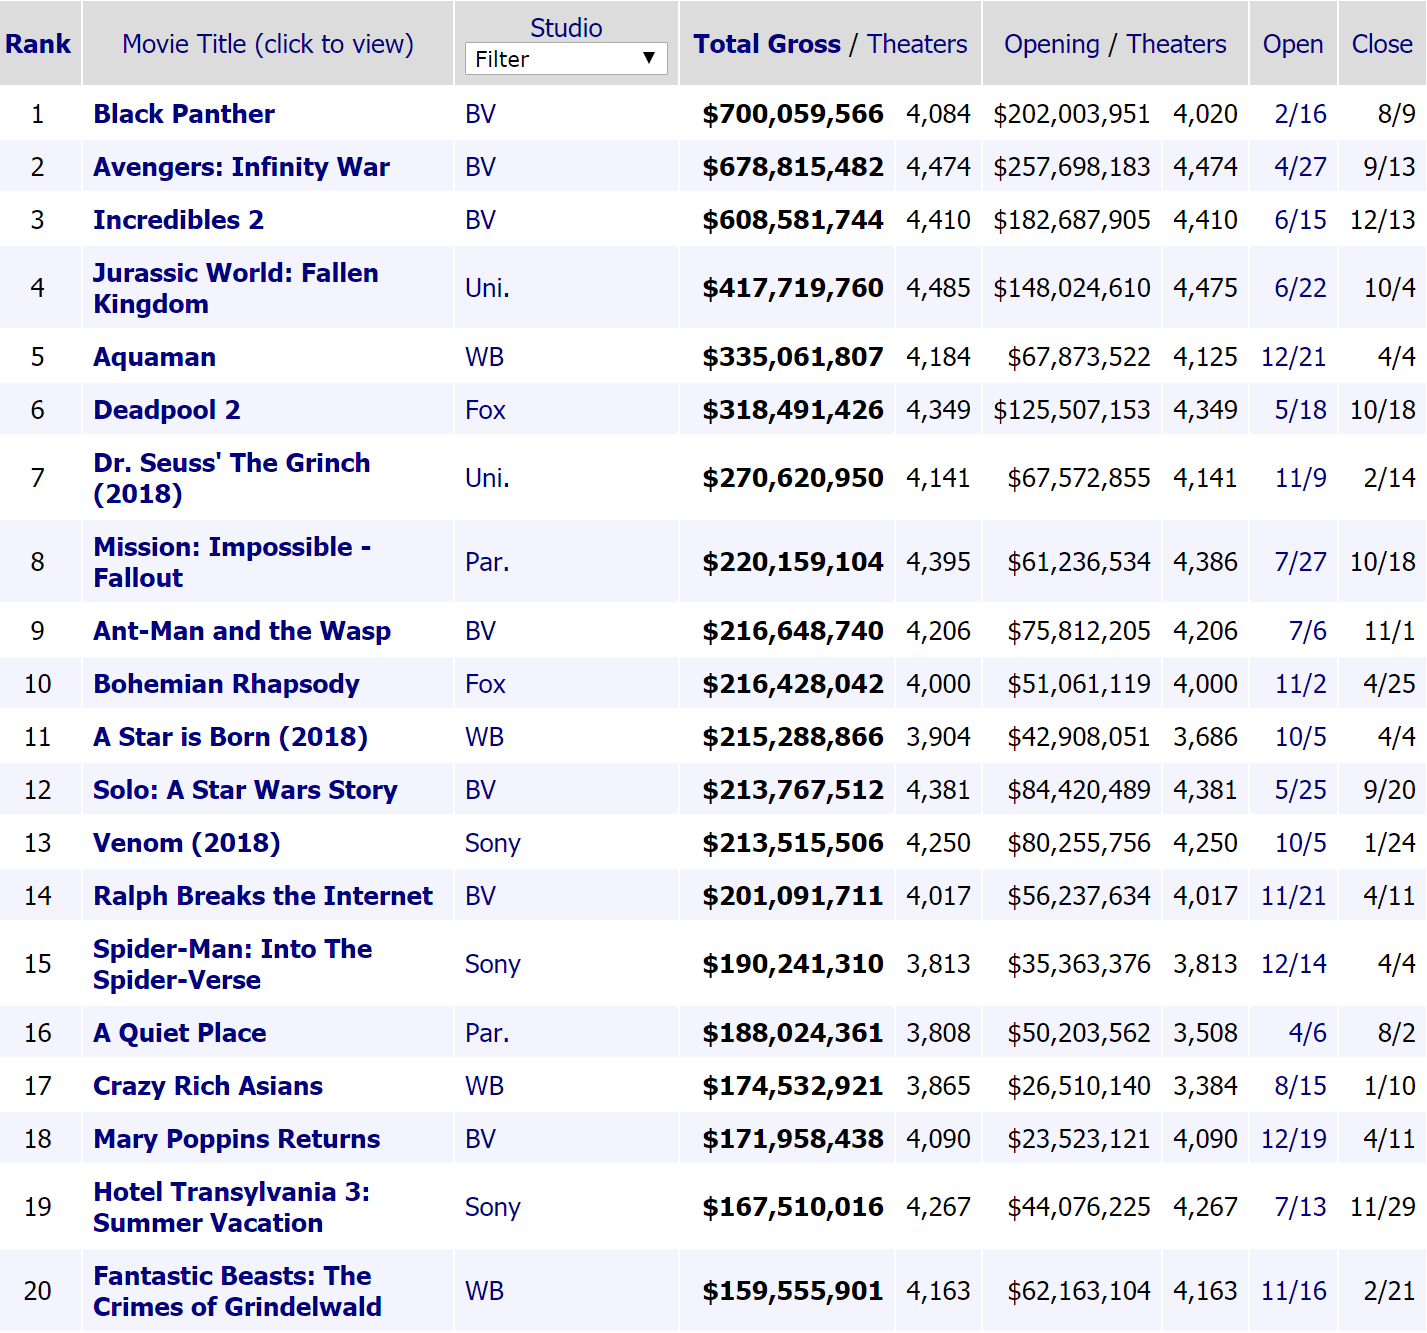
\includegraphics[width=\textwidth]{Topfilms.png}

\vspace{1em}
\textbf{Problems:}
\begin{enumerate}
    \item \underline{The films were released at different numbers of cinemas}
    \vspace{0.5em}
    \\For example, A Quiet Place earnt less than Jurassic World, but was available at 3808 cinemas to Jurassic World’s 4485 cinemas.
    \item \underline{The films were released at different cinemas}
    \vspace{0.5em}
    \\Each cinema sets its own ticket price, and has different deals for cheap Tuesdays, discounts, promotional prices with nearby restaurants, etc. The amount grossed does not give any indication of how many audience members saw the film or the success of the film, because there are no numbers on how many cents of each ticket price is taken by the cinema.
    \item \underline{What year they opened and closed}
    \vspace{0.5em}
    \\This is more a problem with the design of the spreadsheet itself than the design of the project, but the dates for opening and closing are ambiguous. I might guess, looking at the numbers, that the dates are formatted mm/dd, but there is no year on either to show how long they were open for. Even though this list is for 2018, there’s no indication whether it is the opening dates or closing dates that occur in 2018. I might guess opening, just based on my background knowledge of the titles in the list, but then it doesn’t necessarily follow that the closing year is 2019, many films may be in cinemas for over a year. Rocky Horror Picture Show is still being played at cinemas since 1975.
    \item \underline{They were open for different lengths of time}
    \vspace{0.5em}
    \\The Grinch did not perform as well as Incredibles 2, but it had literally half the time within which to earn that money. If the data divided the gross by average grossed per day, this would be a very different spreadsheet
    \item \underline{Biggest problem: They have different production budgets}
    \vspace{0.5em}
    \\If we’re happy to commit to financial earnings being our metric for success, amount grossed is not a logical approach. Financial success should tell you what production companies/directors/actors are the safest financial investments for investing distribution companies, portfolios managers, etc., but this does nothing to show what kind of return these titles made on their investments, only how much money was received. 
    \vspace{0.5em}
    \\For a film like Jurassic Park, ranked #4 due to grossing ~\$418 million, the production budget was ~\$170 million, meaning that the amount earnt by the movie was approximately 245\% of its investment. 
    \vspace{0.5em}
    \\A Quiet Place, for comparison, ranked at #16 for grossing \$188 million, but had a meagre production budget of \$17 million, meaning that the film earnt 1,106\% of its investment.
    \vspace{0.5em}
    \\For Fantastic Beasts: The Crimes of Grindelwald, the production was ~\$200 million, meaning that the film actually LOST \$40 million, and yet is ranked #20 on the most successful films of 2018. 
\end{enumerate}

\newpage\maketitle\textbf{\large{16.08.19 - Transferring the Learning Journal to Overleaf}}

Struggling to work out how to start a new paragraph rather than new line. New line can be done with just two line breaks in the source code without using $\backslash$newline.$\backslash$par just creates new line too.

I found an option to $\backslash$parskip\{1em\}

What's an em?

My word document had a lot of hyperlinks, 
\href{https://www.overleaf.com/learn/latex/Hyperlinks}{here} is a tutorial on making hyperlinks. Now I can insert all the hyperlinks I had in the original document

I'm having a problem with special characters in Overleaf such as \% and \$ and $\backslash$. I worked out you can use a backslash before most of the special characters to stop them from getting formatted in the main document (thanks, Reddit addiction), but that doesn't work on backslashes. I also can't think of a good way to google that, "how to use backslashes in Overleaf" is only getting me how to use them as a function, of course.

\vspace{1cm}
\maketitle\textbf{\large{19.08.19 - Still transferring the Learning Journal to Overleaf}}

Couldn't stay long enough after class to get my questions answered, but found an answer on a forum to insert the $symbol$ of a backslash as \texttt{"\$$\backslash$backslash\$"}.

\texttt{$\backslash$texttt} makes fonts monospace, I'll keep that going from now on.

An "em" is the space an M takes in the current font. That's quite handy because it's a measurement that changes with the font size.

I'm starting to get the hang of how to run Overleaf now. You really just google everything you want to do and there's always a tutorial for it somewhere. 

\begin{addmargin}[1cm]{0cm}
\underline{Problem:}

I'm a bit confused about how to get an image in - I used one for explaining the bad data from my discipline. In Word I just clipped it with the clipping tool and ctrl+Ved to Word. The tutorial seems to have 5 different ways that I understand equally poorly.

\underline{Solution:}

Oh I see, I had to add the package to the preamble. Oh and the directory is the directory on Overleaf, not my directory.
\end{addmargin}

Wow I didn't realise I had a directory, actually I've put this learning journal in a folder called "Scoping Exercise".

Frankly, I'd like to keep these together so I can easily find codes I used elsewhere. I'll just rename the folder to be all-purpose.

I also had a look at indenting entire paragraphs before, I wonder if I just forgot a package in the preamble like for the graphics.

Yes I did.

You can set the width of the image to equal the text width. 

This is getting a lot easier. I've only spent 2:30hrs on the journal today and I transferred the entire thing including this entry I'm making now.

To be honest, I'm really unaware of any situation where this would be faster or easier than a regular word processor but I'm trusting I'll eventually find one!

\end{document}